% No preâmbulo: \usepackage{graphicx,subfigure,caption,placeins}
\FloatBarrier
\section{Avaliação e Resultados}
\label{sec:result}
A avaliação inclui falhas de estado, interrupções lógicas e TLS nativo no Mininet-WiFi. O protótipo usa ML-KEM-512 e ML-DSA-44; o TLS usa X25519MLKEM768, ML-DSA-44 e AES-256-GCM. Comparações de bytes são internas a cada backend, pois seus parâmetros diferem. Manifestos fixam fontes, configurações e critérios. Tempos e escritas no host não medem energia ou desempenho de ESP32.

\subsection{Falhas de Estado e Unicidade de Chave e Nonce}

A primeira campanha reúne 240 traços: seis políticas, quatro falhas e dez repetições, com oito leituras antes e oito após reinício. As falhas são reinício com checkpoint atual, queda de energia modelada, rollback do cliente e checkpoint truncado. Comparam-se checkpoint, persistência por uso, reserva de blocos e chaves novas por completo, PSK e PSK+KEM. Passaram 65 verificações funcionais, incluindo falhas esperadas nos controles vulneráveis.

\begin{figure}[!htb]
\captionsetup{position=bottom,font=small,labelfont=bf}
\setcounter{subfigure}{0}
\centering
\subfigure[Queda de energia modelada.]{
\label{fig:estado_energia}
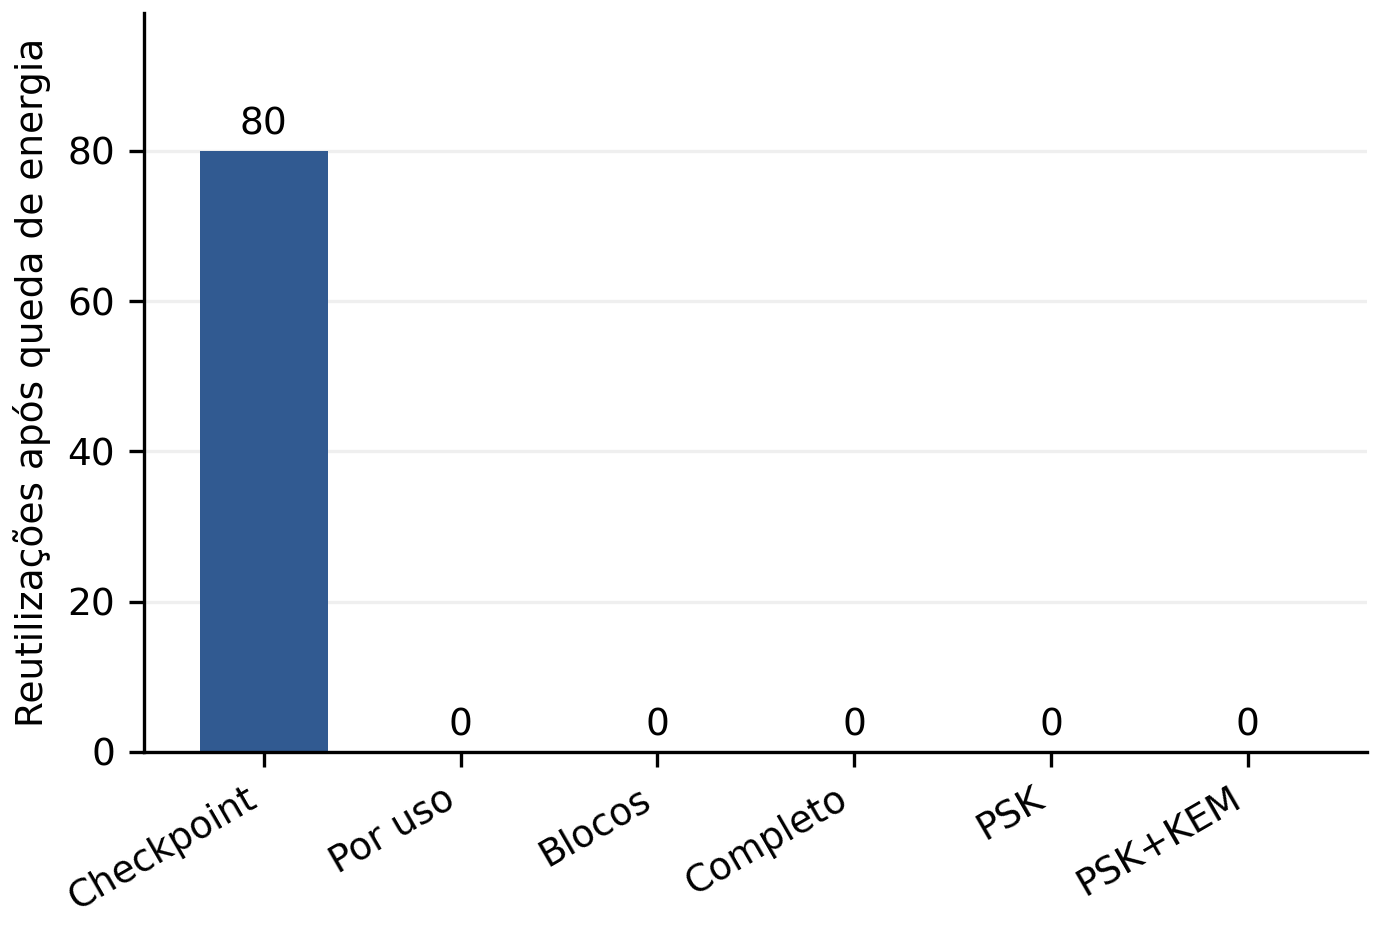
\includegraphics[width=0.46\linewidth]{figuras/avaliacao/estado_energia.png}
}
\subfigure[Rollback do armazenamento.]{
\label{fig:estado_rollback}
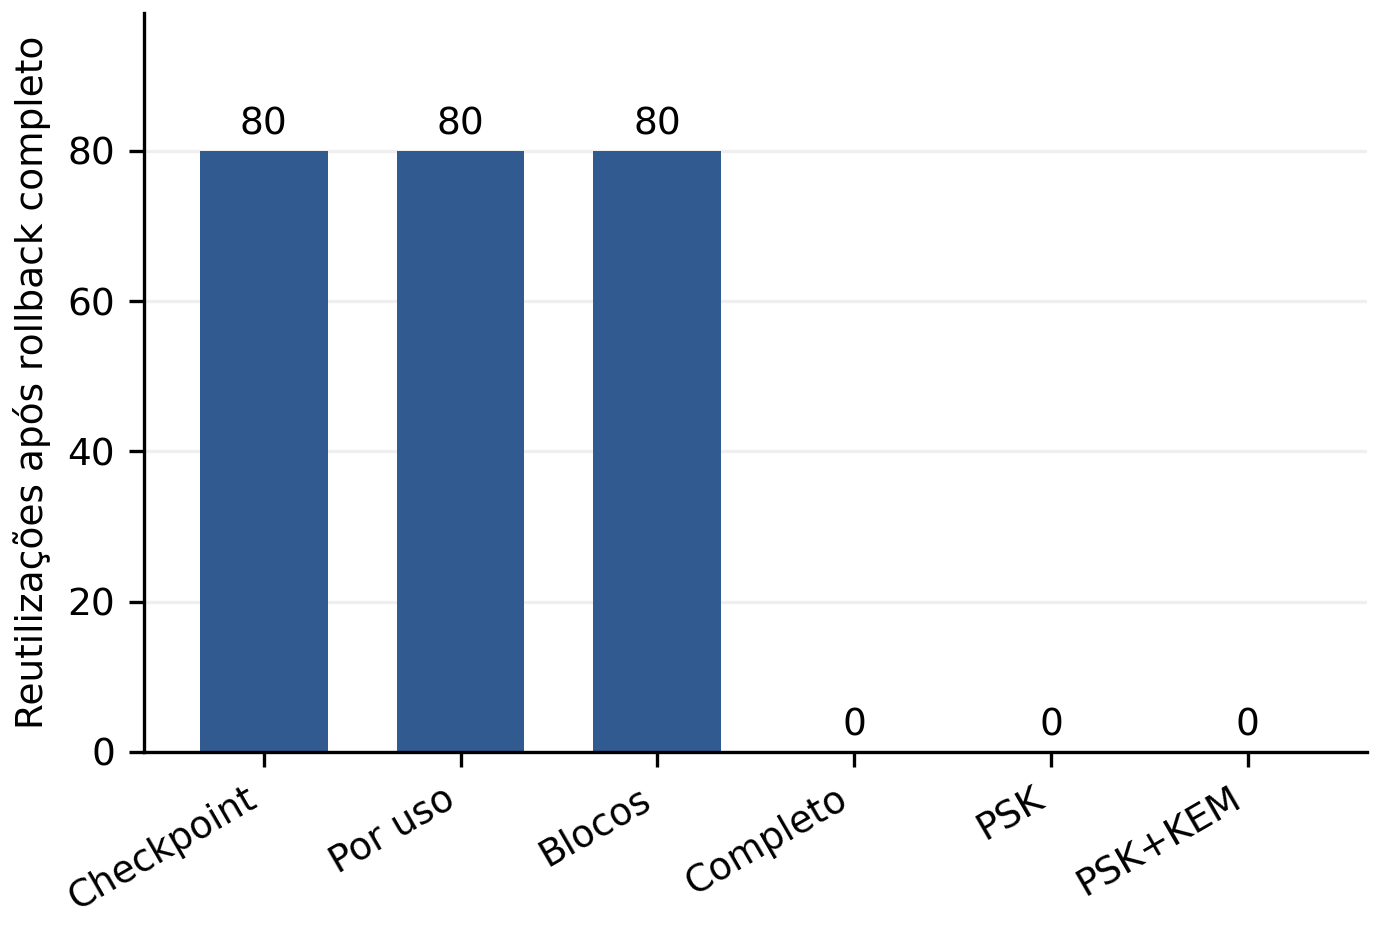
\includegraphics[width=0.46\linewidth]{figuras/avaliacao/estado_rollback.png}
}
\caption{Reutilizações após queda de energia e rollback: totais de dez traços com oito leituras após a falha. Blocos reservam 32 posições; PSK+KEM utiliza ML-KEM novo.}
\label{fig:estado_resultados}
\end{figure}

A Figura~\ref{fig:estado_resultados} mostra os efeitos dessas escolhas. O checkpoint antigo produziu 80 reutilizações após a queda modelada; persistência por uso e reserva de blocos evitaram essa falha com journal atual. Ao restaurar também o journal, as três políticas de contador apresentaram 80 reutilizações cada. Os modos com chave nova apresentaram zero nos cenários testados.

\begin{figure}[!htb]
\captionsetup{position=bottom,font=small,labelfont=bf}
% A figura já tem número na parte anterior; manter os subpainéis nesse número.
\ContinuedFloat
\figuretopcaptrue
\setcounter{subfigure}{2}
\centering
\subfigure[Textos recuperados no rollback.]{
\label{fig:estado_textos}
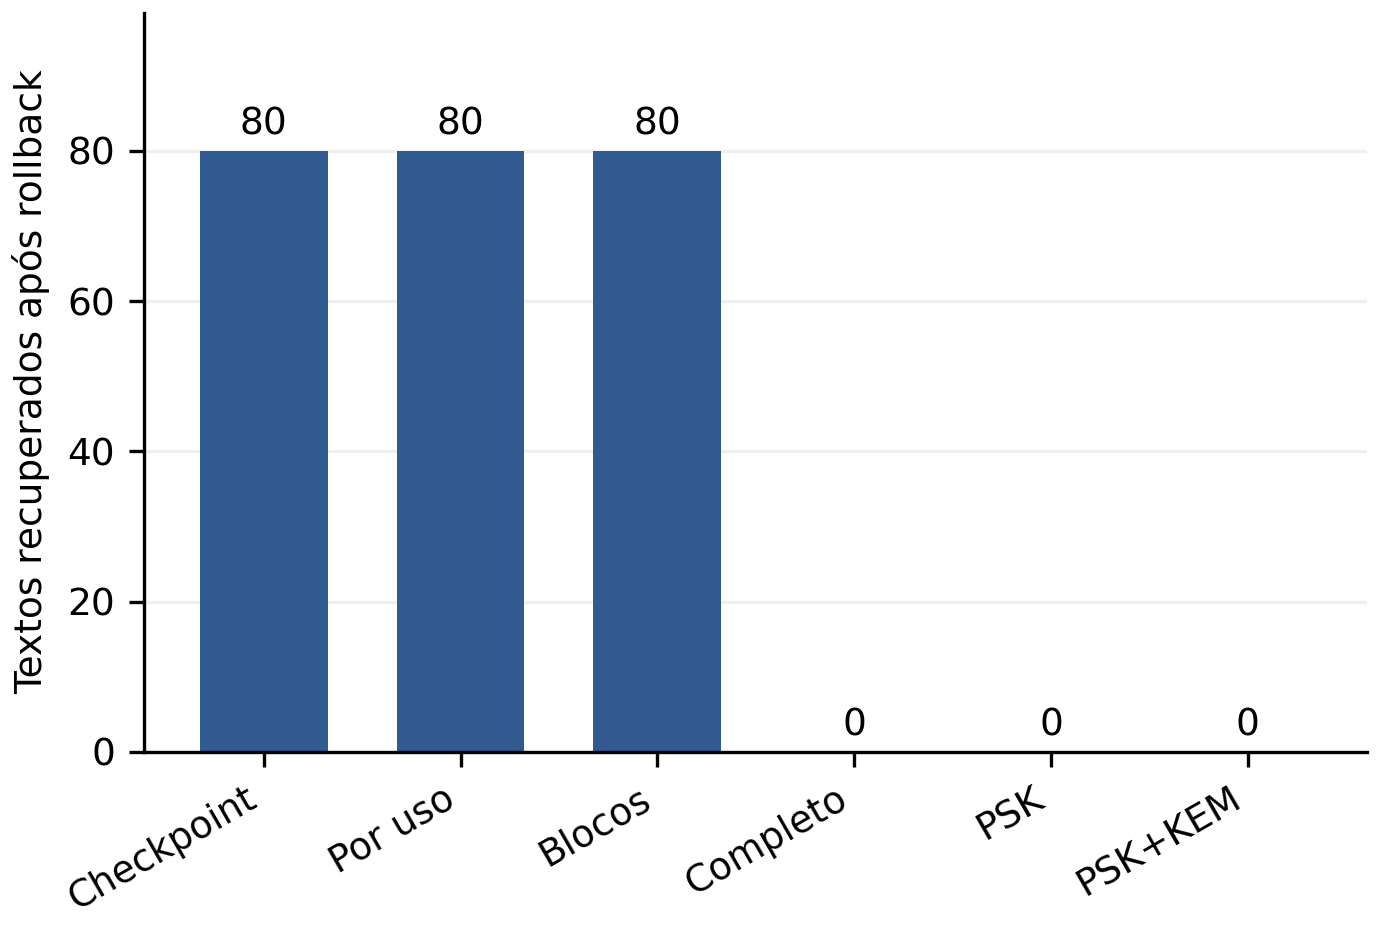
\includegraphics[width=0.46\linewidth]{figuras/avaliacao/estado_textos.png}
}
\subfigure[Escritas na fase estável.]{
\label{fig:estado_escritas}
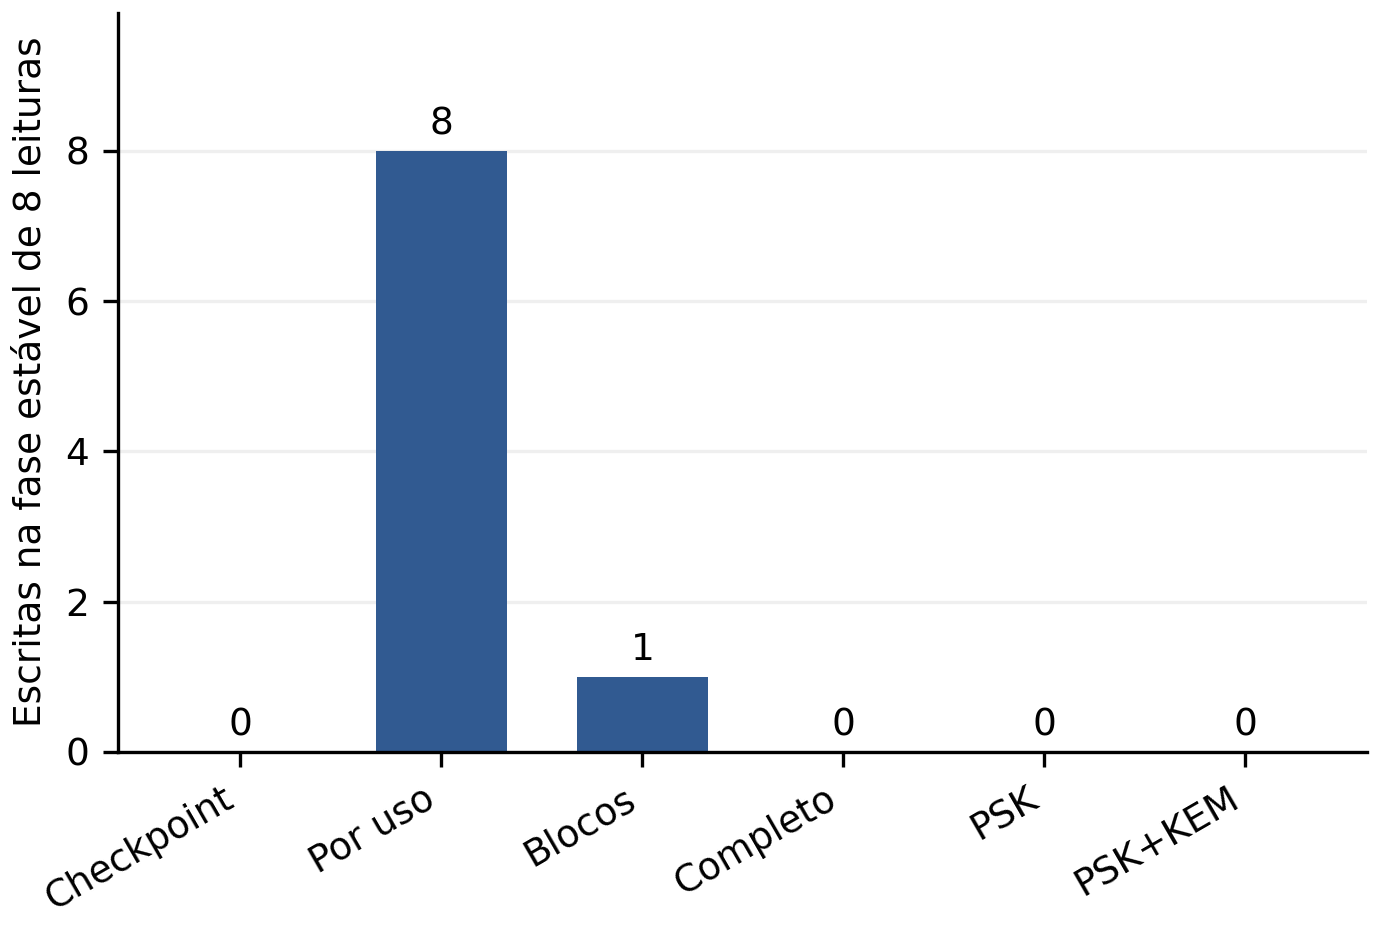
\includegraphics[width=0.46\linewidth]{figuras/avaliacao/estado_escritas.png}
}
\caption{Reutilizações e textos (continuação): (c) textos recuperados no rollback, total de dez traços; (d) mediana de escritas por traço na fase estável com oito leituras.}
\label{fig:estado_resultados_continuacao}
\end{figure}

O controle de texto conhecido recuperou 80 leituras por política vulnerável no rollback. Embora o gateway rejeite registros repetidos, a exposição já existia no tráfego cifrado. Nas oito leituras estáveis, a persistência por uso realizou oito escritas e a reserva de blocos realizou uma; esses contadores excluem inicialização e checkpoints do boot. Persistir contadores protege contra perda de energia com registro atual, mas não contra restauração integral desse registro.

\subsection{Interrupções, Fallback e Confirmação Perdida}

A segunda campanha inclui 330 casos: onze cenários, três modos com chave nova e dez repetições. A Figura~\ref{fig:transicoes_resultados} apresenta custos e efeitos das interrupções. Os pontos A--K correspondem a fluxo sem falha; interrupção após ClientHello, ServerHello, ClientFinished, commit do gateway, confirmação de chave, checkpoint e cifragem da leitura; ACK perdido; checkpoint truncado; e raiz perdida no gateway. A matriz usa transporte lógico e primitivas reais; não mede perda de pacotes.

\begin{figure}[!htb]
\captionsetup{position=bottom,font=small,labelfont=bf}
\setcounter{subfigure}{0}
\centering
\subfigure[Bytes por ponto de interrupção.]{
\label{fig:transicoes_bytes}
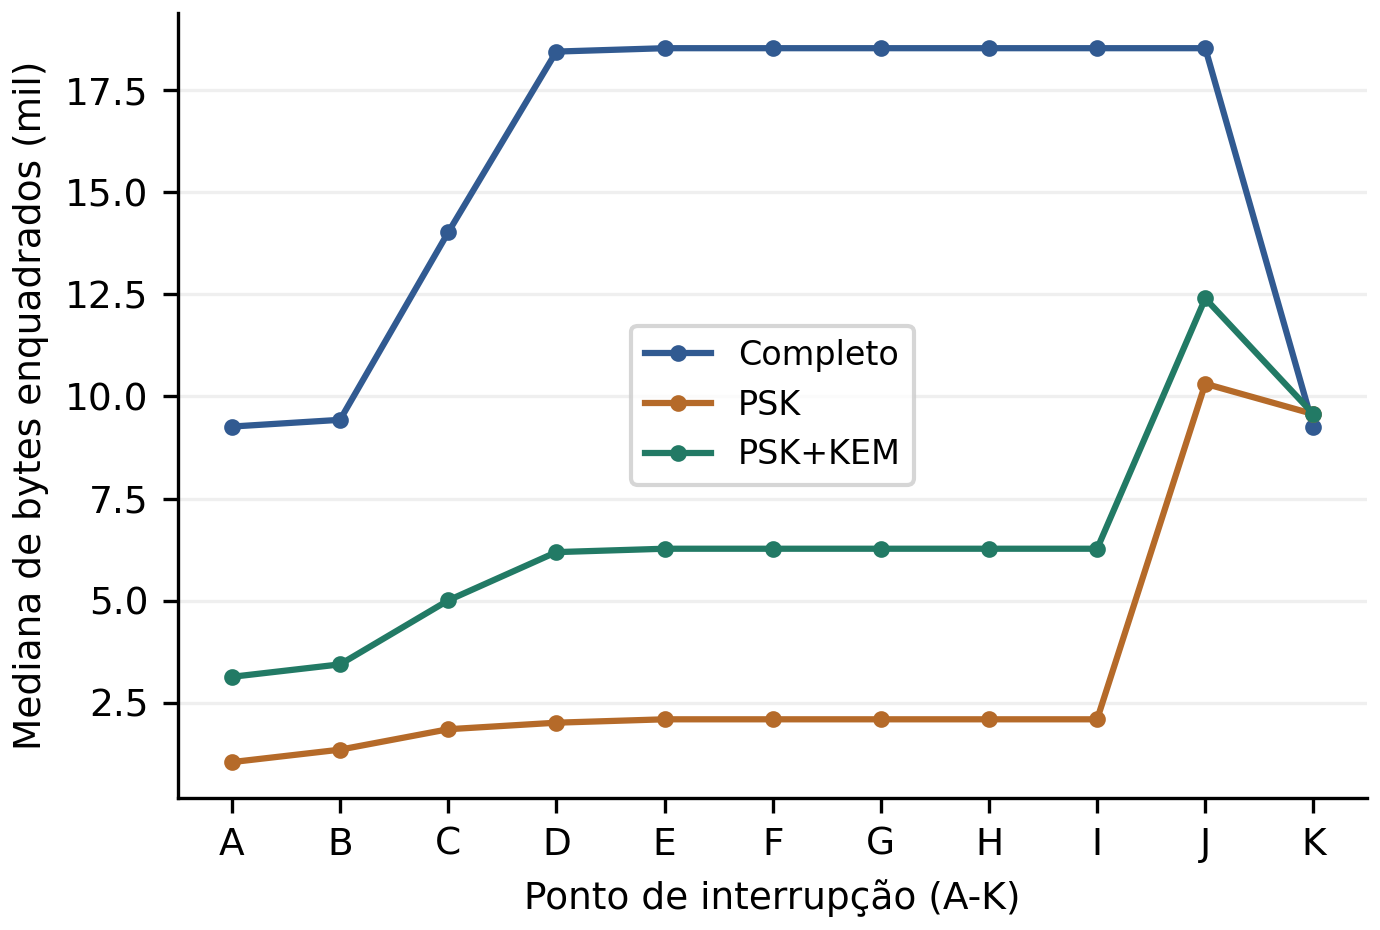
\includegraphics[width=0.46\linewidth]{figuras/avaliacao/transicoes_bytes.png}
}
\subfigure[Fallbacks com PSK+KEM.]{
\label{fig:transicoes_fallbacks}
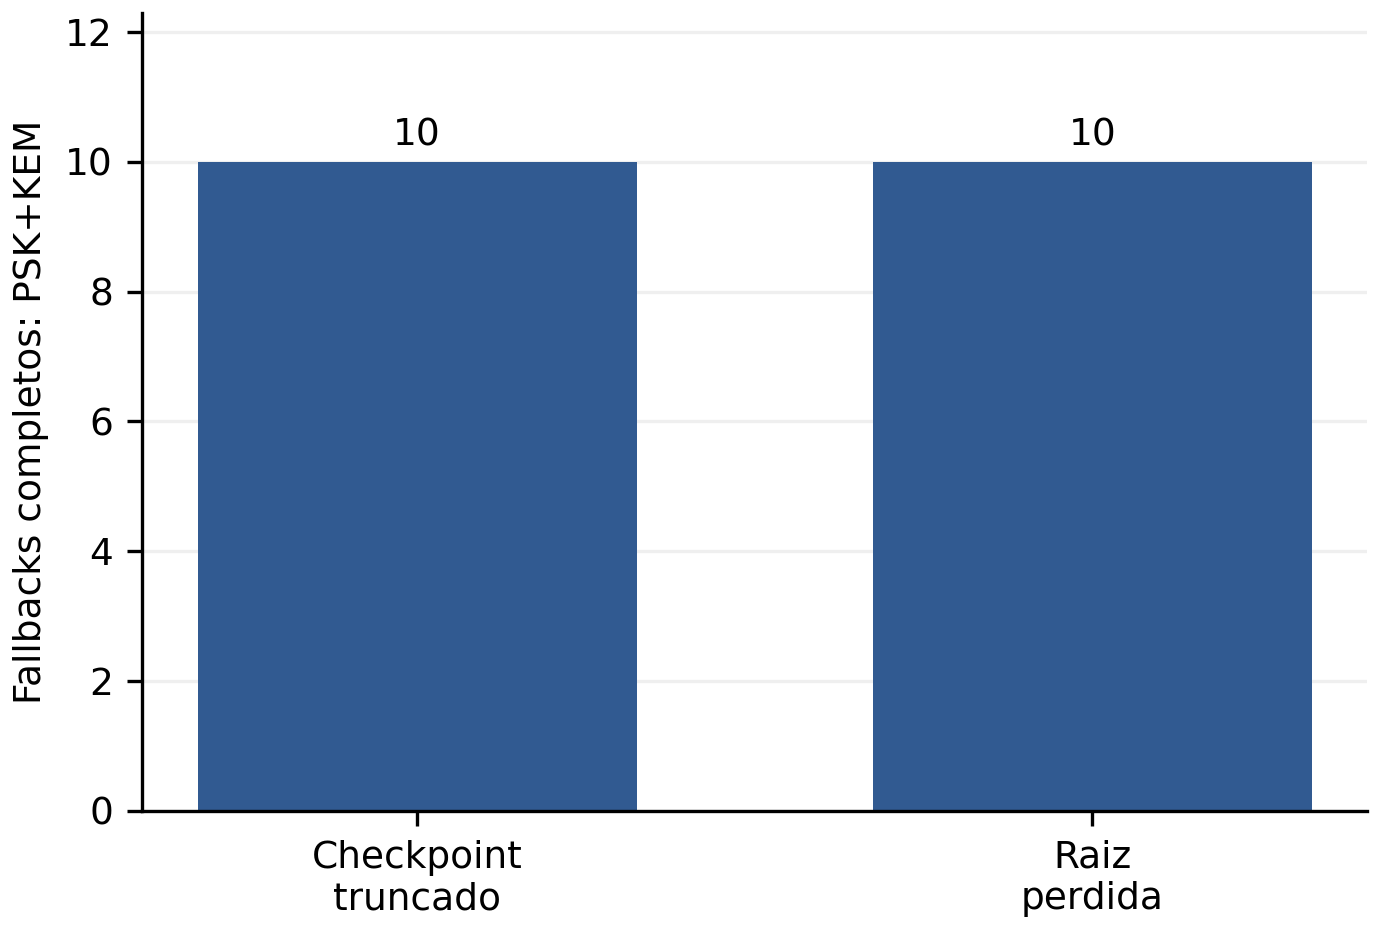
\includegraphics[width=0.46\linewidth]{figuras/avaliacao/transicoes_fallbacks.png}
}
\caption{Protocolo experimental: (a) mediana de bytes de dez repetições; (b) total de fallbacks. A--K seguem a ordem descrita no texto. Esses bytes não representam TLS.}
\label{fig:transicoes_resultados}
\end{figure}

Sem falha, o handshake completo custou 9.263 bytes e a retomada com ML-KEM custou 3.136 bytes, redução de 66,14\%. Com a raiz perdida, a tentativa de retomada seguida de autenticação completa custou 9.568 bytes, contra 9.263 do modo completo: acréscimo de 3,29\%. A hipótese de economia universal foi, portanto, refutada. Os bytes incluem mensagens enquadradas das tentativas e confirmações perdidas; excluem bootstrap, leituras e cabeçalhos IP. O transporte não envia uma mensagem de erro para o pedido rejeitado.

\begin{figure}[!htb]
\captionsetup{position=bottom,font=small,labelfont=bf}
% A figura já tem número na parte anterior; manter os subpainéis nesse número.
\ContinuedFloat
\figuretopcaptrue
\setcounter{subfigure}{2}
\centering
\subfigure[Economia condicionada ao estado.]{
\label{fig:transicoes_economia}
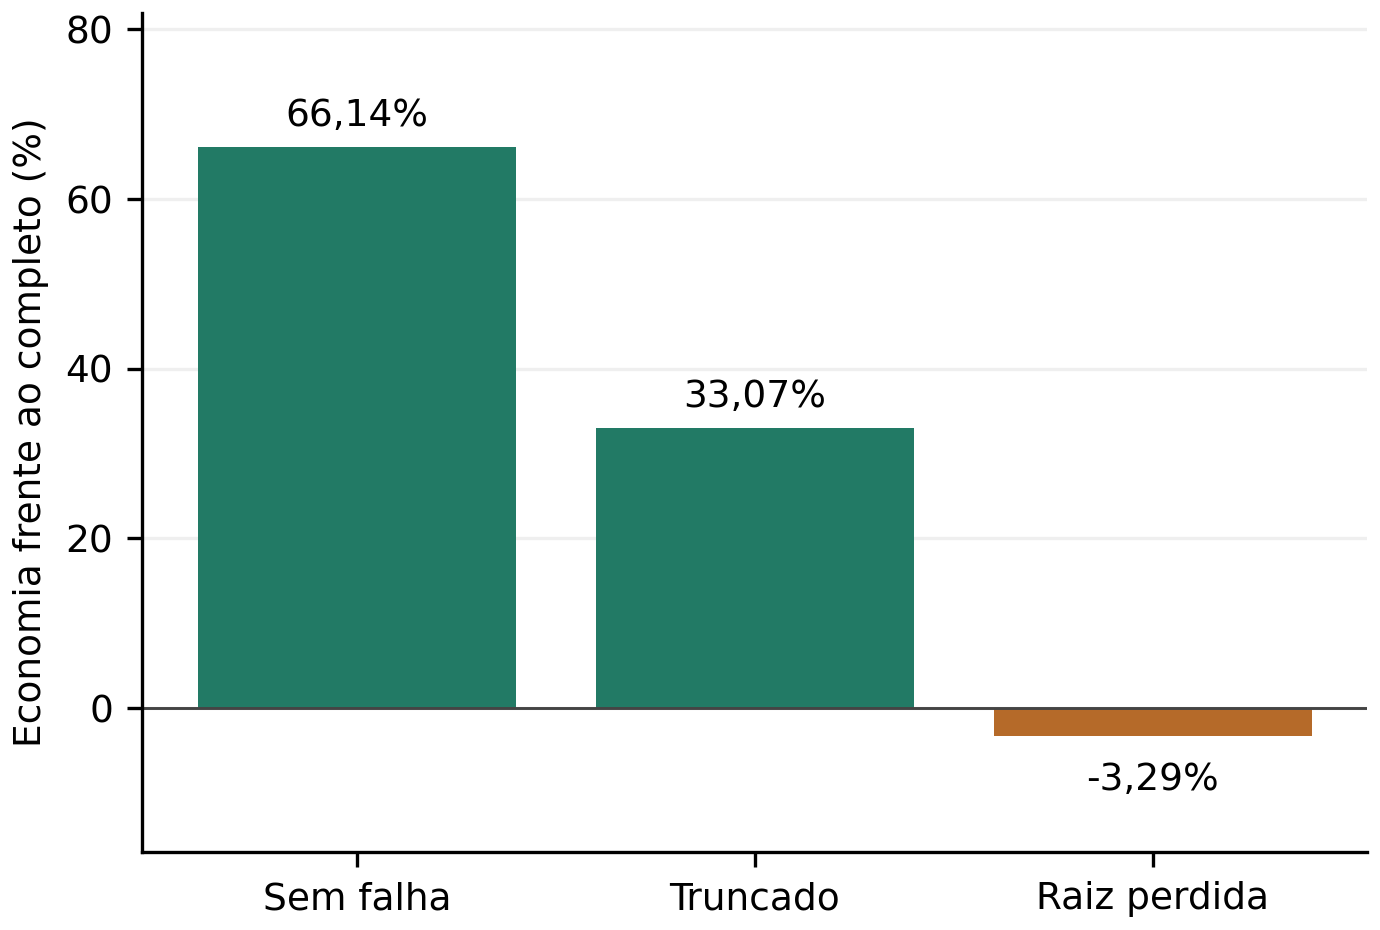
\includegraphics[width=0.46\linewidth]{figuras/avaliacao/transicoes_economia.png}
}
\subfigure[Duplicação após ACK perdido.]{
\label{fig:transicoes_duplicados}
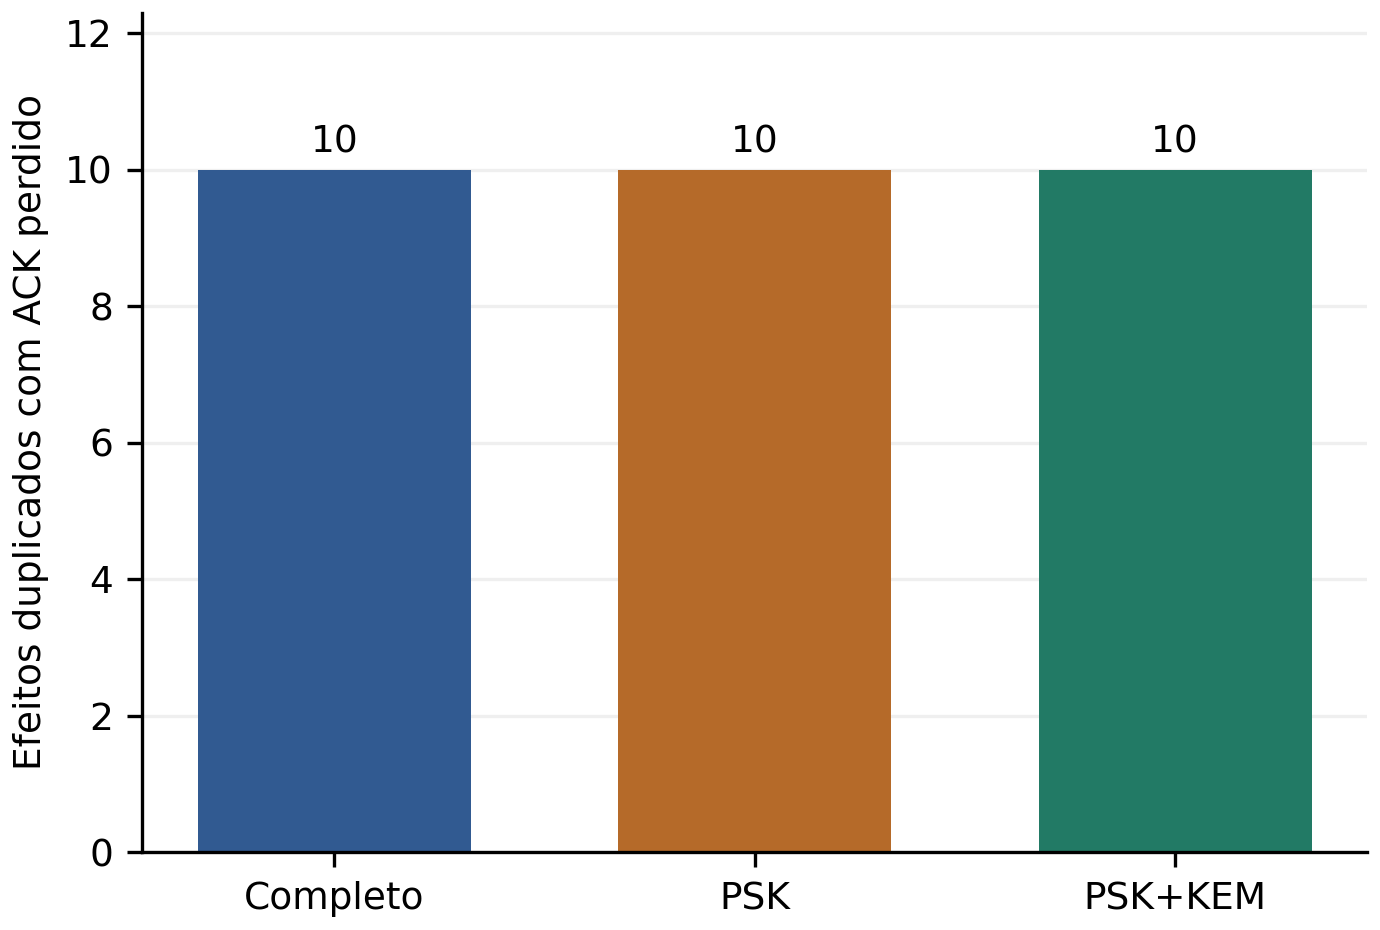
\includegraphics[width=0.46\linewidth]{figuras/avaliacao/transicoes_duplicados.png}
}
\caption{Protocolo experimental (continuação): (c) economia de bytes, mediana de dez repetições; (d) total de efeitos duplicados após ACK perdido.}
\label{fig:transicoes_resultados_continuacao}
\end{figure}

Os modos com chave nova atenderam aos critérios de unicidade e recuperação após uma falha seguida de tentativa sem interrupção. O ACK perdido produziu dez efeitos duplicados por modo na aplicação sem ledger, apesar das chaves novas. Repetição da leitura e replay criptográfico são, portanto, propriedades distintas.

\subsection{Custos e Deduplicação com TLS}

O piloto usa OpenSSL 3.5.9, um sensor Wi-Fi emulado e um gateway. 0-RTT foi desativado. Perdas netem de 0\%, 1\% e 5\% e atraso de 2 ms são aplicados por direção no enlace AP--servidor. Cinco blocos, dois modos TLS e deduplicação ativa/desativada totalizam 60 condições. Cada condição tem cinco leituras e seis processos, devido ao ACK perdido: 360 processos e 300 entregas lógicas. Os IDs se repetem entre comparadores; as entregas não são amostras independentes. A ordem rotaciona, mas as perdas não são exatamente pareadas.

\begin{figure}[!htb]
\captionsetup{position=bottom,font=small,labelfont=bf}
\setcounter{subfigure}{0}
\centering
\subfigure[Handshake com contexto disponível.]{
\label{fig:tls_handshake}
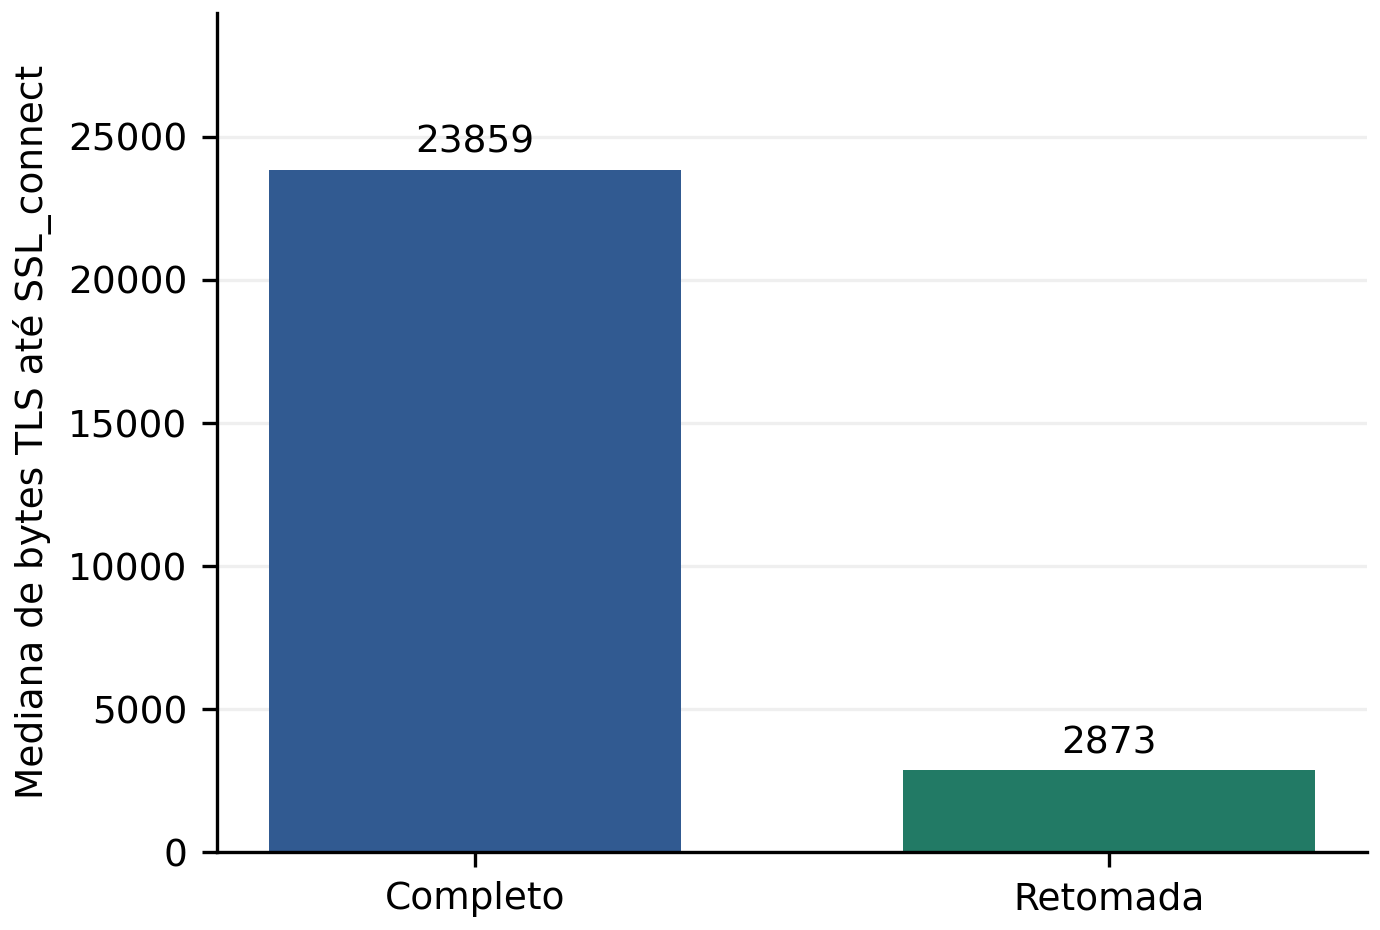
\includegraphics[width=0.46\linewidth]{figuras/avaliacao/tls_handshake.png}
}
\subfigure[Tráfego IPv4 por ensaio.]{
\label{fig:tls_ipv4}
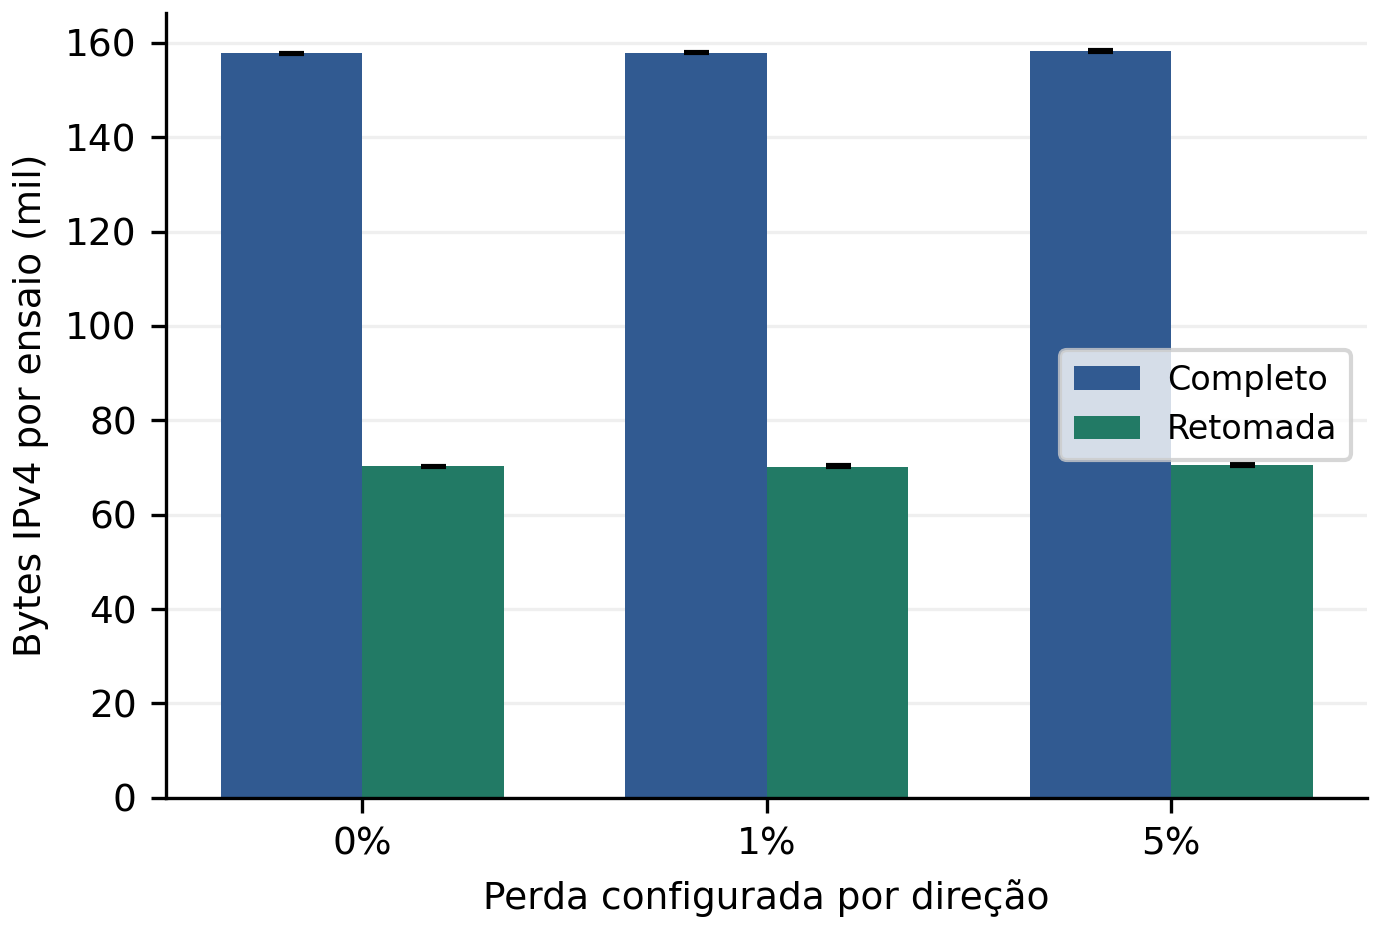
\includegraphics[width=0.46\linewidth]{figuras/avaliacao/tls_ipv4.png}
}
\caption{Custos no piloto TLS: (a) mediana do handshake quente; (b) tráfego IPv4 por ensaio com deduplicação ativa, cinco blocos por configuração. Hastes indicam mínimo e máximo, não intervalos de confiança.}
\label{fig:tls_resultados}
\end{figure}

O gateway reinicia antes da terceira leitura, perdendo o cache e preservando o ledger. A quarta perde o ACK após commit e é repetida; a quinta restaura o ticket salvo após a terceira. O modo de retomada realiza dois handshakes completos e quatro retomados por condição, contra seis completos no comparador. Houve 30 fallbacks e 30 retomadas com ticket restaurado. Verificaram-se parâmetros e compartilhamentos públicos novos; não foram exportadas chaves ou IVs internos do TLS.

Na Figura~\ref{fig:tls_resultados}, no segundo boot, com contexto disponível, o handshake completo teve mediana de 23.859 bytes TLS e a retomada, 2.873 bytes: redução de 87,96\%. O intervalo termina no retorno de SSL\_connect e exclui tickets pós-handshake, cabeçalhos IP e demais conexões do ensaio. Com deduplicação ativa, as medianas de bytes IPv4 por ensaio foram 157.895 contra 70.250 em 0\%, 157.895 contra 70.158 em 1\% e 158.287 contra 70.550 em 5\%, para completo e retomada. Os totais incluem tentativas e encerramentos observados no servidor.

\begin{figure}[!htb]
\captionsetup{position=bottom,font=small,labelfont=bf}
% A figura já tem número na parte anterior; manter os subpainéis nesse número.
\ContinuedFloat
\figuretopcaptrue
\setcounter{subfigure}{2}
\centering
\subfigure[Tempo até confirmação da leitura.]{
\label{fig:tls_ack}
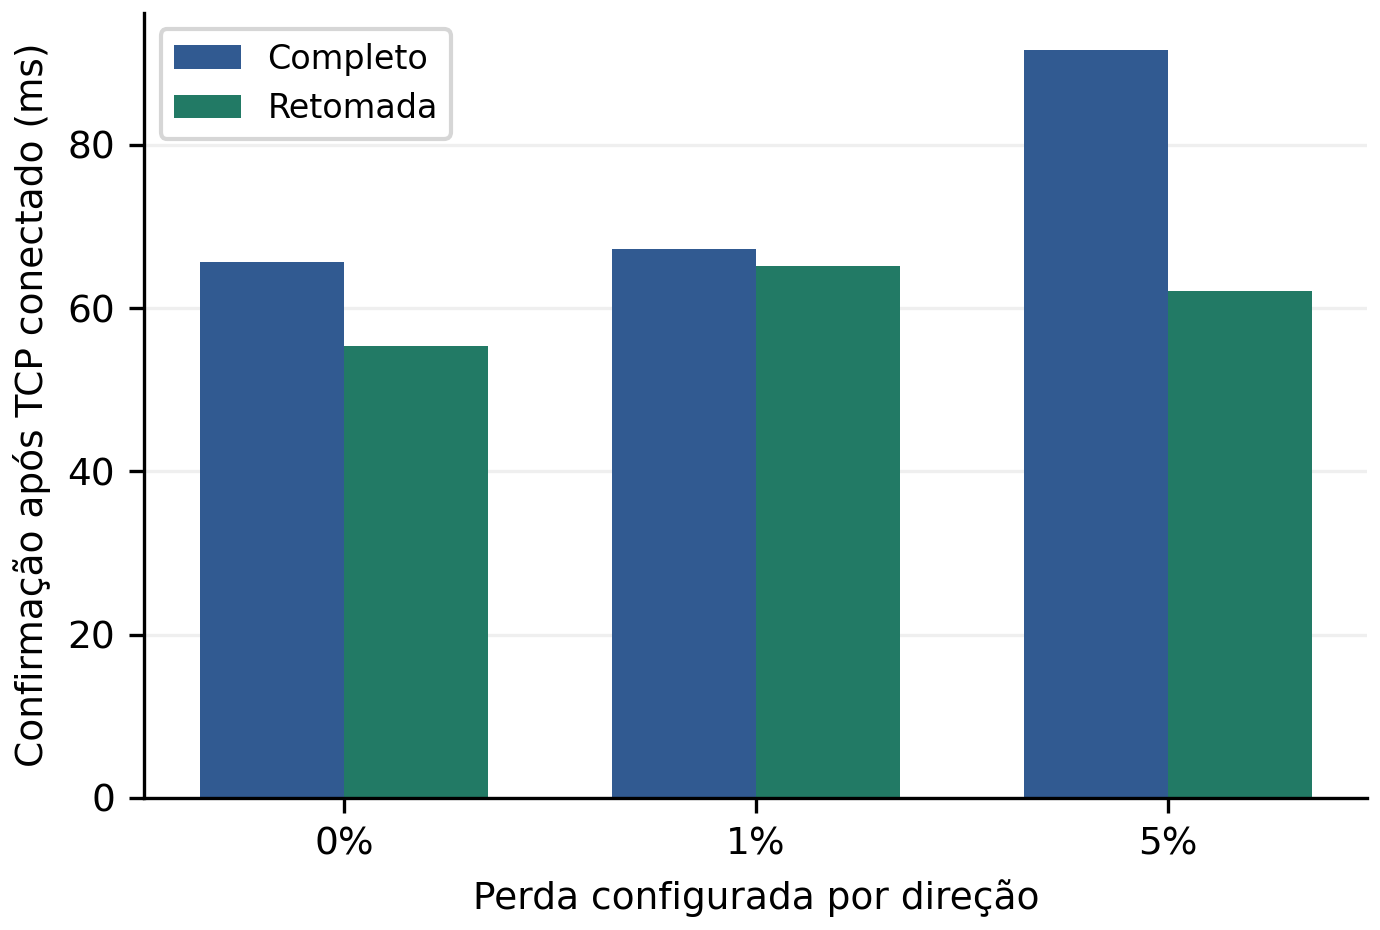
\includegraphics[width=0.46\linewidth]{figuras/avaliacao/tls_ack.png}
}
\subfigure[Recuperação no host.]{
\label{fig:tls_recuperacao}
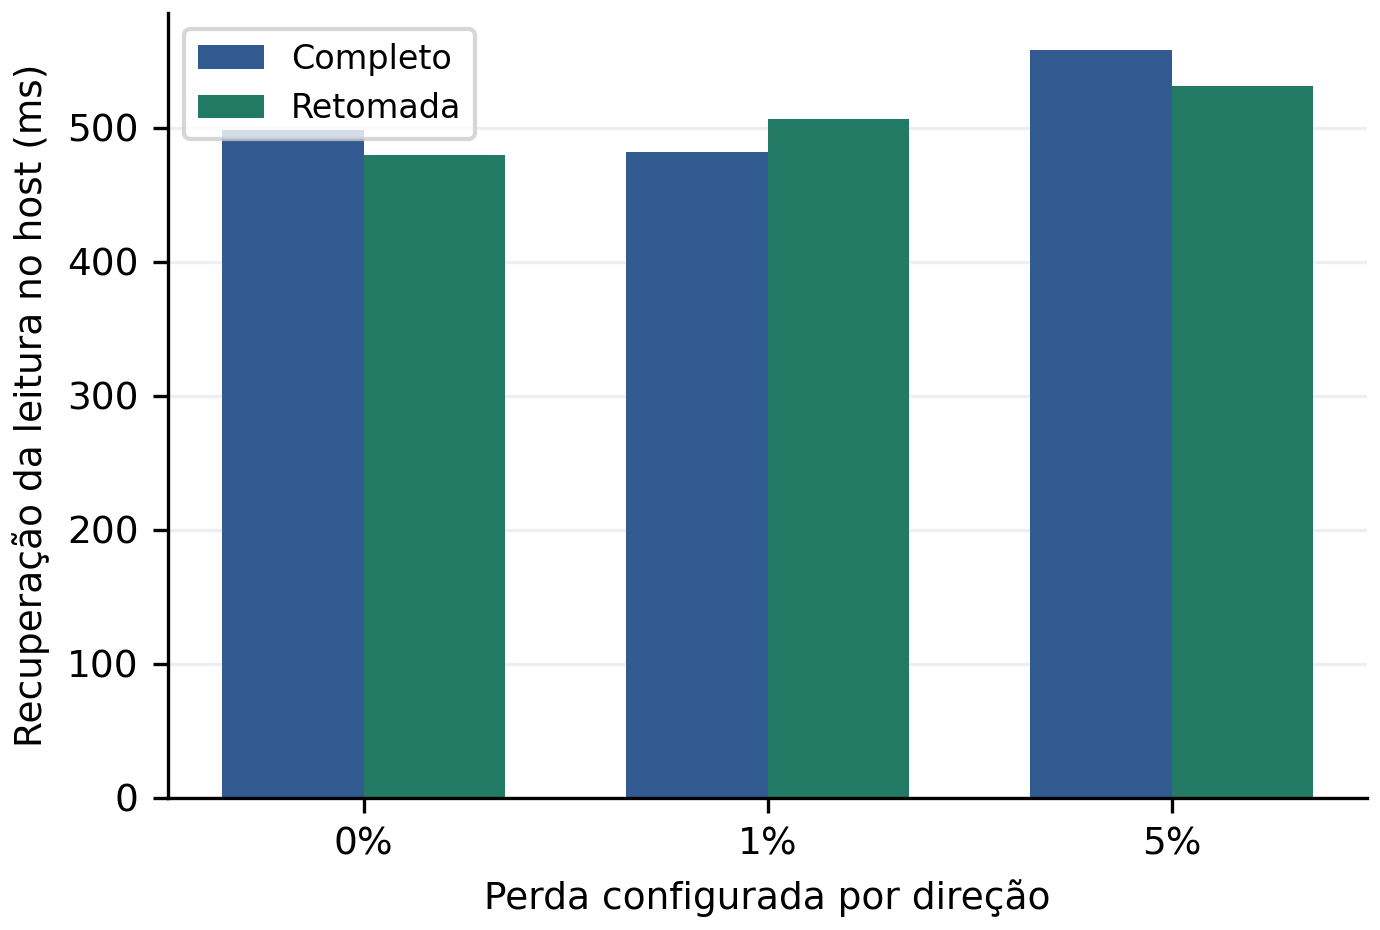
\includegraphics[width=0.46\linewidth]{figuras/avaliacao/tls_recuperacao.png}
}
\caption{Custos no piloto TLS (continuação): (c--d) deduplicação ativa, cinco blocos por configuração. Tempos são medianas das medianas por bloco.}
\label{fig:tls_resultados_continuacao}
\end{figure}

As medianas de confirmação após TCP conectado foram 65,7/55,4 ms, 67,2/65,2 ms e 91,6/62,1 ms para completo/retomada em 0\%, 1\% e 5\%, com ledger. São medianas das medianas por bloco. Recuperação inclui processos e repetição após ACK perdido. TCP\_INFO conta retransmissões nos endpoints antes de fechar; o PCAP pode perder a primeira cópia descartada. Encerramentos também entram, inclusive em 0\%. Cinco blocos não sustentam P95 robusto ou superioridade estatística geral.

\begin{figure}[!htb]
\captionsetup{position=bottom,font=small,labelfont=bf}
\setcounter{subfigure}{0}
\centering
\subfigure[Retransmissões TCP.]{
\label{fig:tls_retransmissoes}
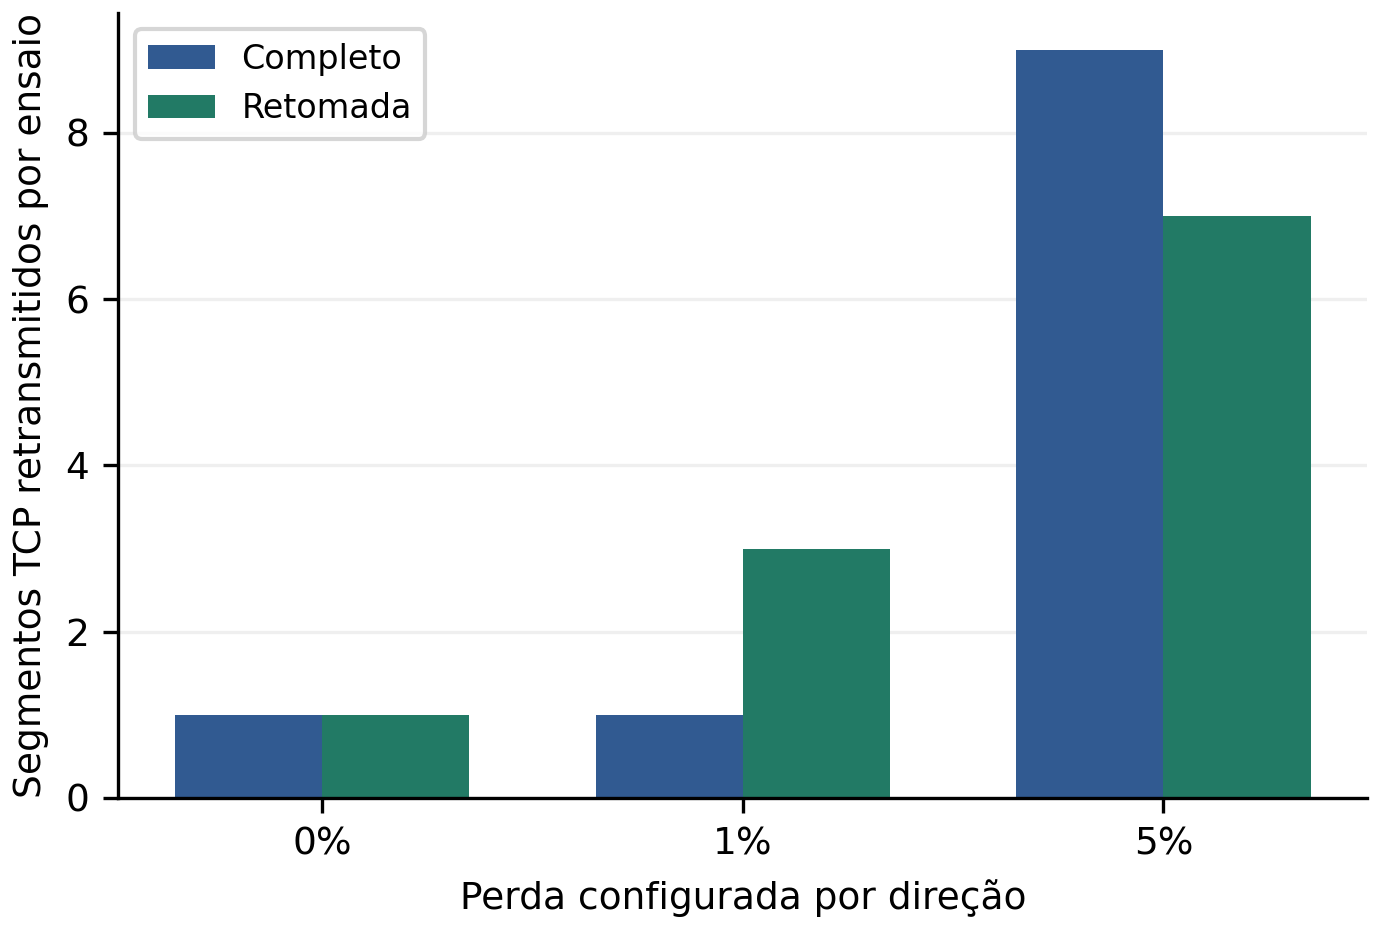
\includegraphics[width=0.46\linewidth]{figuras/avaliacao/tls_retransmissoes.png}
}
\subfigure[Efeitos duplicados no banco.]{
\label{fig:tls_duplicados}
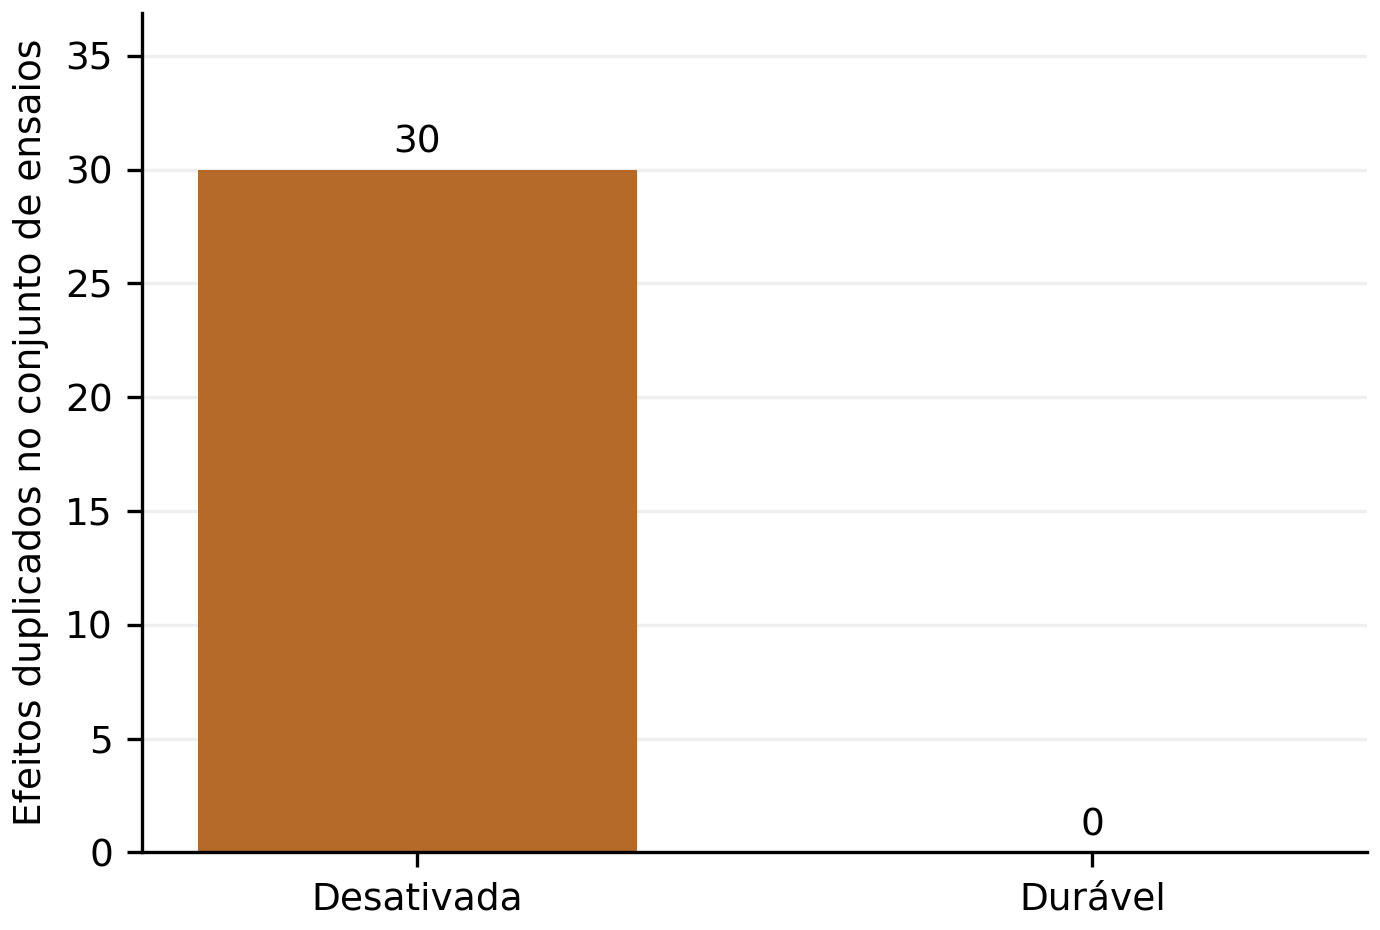
\includegraphics[width=0.46\linewidth]{figuras/avaliacao/tls_duplicados.png}
}
\caption{Retransmissões e deduplicação no piloto TLS: (a) mediana de retransmissões TCP por ensaio com deduplicação ativa, cinco blocos por configuração; (b) efeitos duplicados nas 30 condições de cada modo de deduplicação.}
\label{fig:tls_controles}
\end{figure}

A Figura~\ref{fig:tls_controles} reúne retransmissões e efeitos duplicados. O controle acumulou 30 efeitos duplicados, contra zero com ledger durável. Ambos rastreiam IDs e rejeitam conflitos; muda apenas a supressão. SQLite persiste leitura e efeito antes do ACK. Restaurar todo o banco desfaz essa proteção no controle separado. O recorte não estabelece execução única de atuadores, resistência a rollback conjunto ou economia energética em hardware físico.

\FloatBarrier
